\documentclass[floatfix,nofootinbib,superscriptaddress,fleqn]{revtex4-2} 
%\documentclass[aps,epsfig,tightlines,fleqn]{revtex4}
\usepackage[utf]{kotex}
\usepackage[HWP]{dhucs-interword}
\usepackage[dvips]{color}
\usepackage{graphicx}
\usepackage{bm}
%\usepackage{fancyhdr}
%\usepackage{dcolumn}
\usepackage{defcolor}
\usepackage{amsmath}
\usepackage{amsfonts}
\usepackage{amssymb}
\usepackage{amscd}
\usepackage{amsthm}
\usepackage[utf8]{inputenc}
 \usepackage{setspace}
%\pagestyle{fancy}

\begin{document}

\title{\Large 2022년 1학기 물리학 I: Quiz 11}
\author{김현철\footnote{Office: 5S-436D (면담시간 매주
    화요일-16:00$\sim$20:00)}} 
\email{hchkim@inha.ac.kr}
\author{Lee Hui-Jae} 
\email{hjlee6674@inha.adu}
\affiliation{Hadron Theory Group, Department of Physics,
Inha University, Incheon 22212, Republic of Korea }
\date{Spring semester, 2022}



\maketitle


\noindent {\bf 문제 1. (40 pt) (복습문제)} 
그림~\ref{fig:1}처럼 질량이 $m=0.140$ 
kg, 높이 $H=12$ cm인 금속 깡통은 균일한 물질로 되어 있다. 
\begin{figure}[htp]
  \centering
  \includegraphics[scale=0.5]{Qfig10-3-20210402.png}  
  \caption{문제 1}
  \label{fig:1}
\end{figure}
깡통 안에는 질량이 0.210 kg인 콜라가 채워져 있다. 이 깡통의 위쪽과
아래쪽에 작은 구멍을 뚫으면 콜라가 빠진다. 구멍 때문에 손실된 금속의
질량은 무시할 만하다고 하자.
\begin{itemize}
\item[(가)] 처음과
\item[(나)] 콜라가 모두 빠진 다음에 깡통과 콜라의 질량 중심의 높이
  $h$는 각각 얼마인가?
\item[(다)] 콜라가 빠지면서 $h$는 어떻게 변화하는가?
\item[(라)] $x$를 남아있는 콜라의 높이라고 하면, 질량중심이 가장 낮은
  점에 있을 때의 $x$ 값을 구하여라. 
\end{itemize}
\noindent {\bf 풀이 : } 
\begin{itemize}
  \item[(가)] 깡통 바닥의 중심을 원점으로 하자. $A$를 깡통 옆면의 넓이라고 하면 
  깡통 옆면의 질량 중심의 높이는,
  \begin{align}
    z_{cm} =\frac{1}{M}\int z\,dM=\frac{1}{A}\int z\,dA,\,\,\, A =2\pi R z,
  \end{align}
  를 통해 계산할 수 있다. $R$은 깡통 바닥의 반지름이다.
   $V$를 콜라의 부피라고 하면 콜라의 질량 중심의 높이는,
  \begin{align}
    z_{cm} =\frac{1}{m}\int z\,dm=\frac{1}{V}\int z\,dV,\,\,\,V=\pi R^2 z,
  \end{align}
  를 통해 계산할 수 있다. 따라서 $M$을 깡통의 질량, $m$을 콜라의 질량이라 하면 
  전체 질량 중심의 높이 $h$는,
  \begin{align}
    \begin{split}
      h &= \frac{1}{M+m}\left(\frac{M}{A}\int z\,dA
      +\frac{m}{V}\int z\,dV\right) \\
       &= \frac{1}{M+m}\left(\frac{M}{2\pi R H}\int_0^H 2\pi R z\,dz
      +\frac{m}{\pi R^2 H}\int_0^H\pi R^2 z\,dz\right)  \\
      &= \frac{1}{M+m}\left(\frac{M}{H}\int_0^H z\,dz
      +\frac{m}{H}\int_0^H z\,dz\right) \\
      &= \frac{1}{M+m}\left(
        \frac{M}{H}\frac{1}{2}H^2
        +\frac{m}{H}\frac{1}{2}H^2
      \right)  \\
      &=\frac{1}{2}H,
    \end{split}
  \end{align}
  이다. $H=12$ cm이므로 전체 질량 중심의 높이는 6 cm 이다.
  \item[(나)] 콜라가 모두 빠져 나갔으므로 $h$는,
  \begin{align}
    \begin{split}
      h&=\frac{1}{V}\int z\,dV 
      = \frac{1}{2\pi R H}\int_0^H 2\pi R z\,dz \\
      &=\frac{1}{H}\int_0^H z\,dz \\
      &=\frac{1}{2}H,
    \end{split}
  \end{align}
  이다. 따라서 콜라가 모두 빠져나가도 전체 질량 중심의 높이는 6 cm 이다.
  \item[(다)] 콜라가 빠져나갈 때 콜라의 높이를 $x$라고 하자. 콜라의 높이는 
  더 이상 $H$가 아니고 깡통 안에 남은 콜라의 질량 $m$도 상수가 아니다. 콜라가 
  가득 차 있을 때의 질량을 $m_0$,
  콜라의 밀도를 $\rho$라고 하면,
  \begin{align}
    \begin{split}
      \rho = \frac{m_0}{\pi R^2 H}
    \end{split}
  \end{align}
  이고 깡통 안에 남은 콜라의 질량 $m$은,
  \begin{align}\label{eq:1-1}
    m= \rho\pi R^2 x = \frac{m_0x}{H}
  \end{align}
  이다.
  전체 질량 중심의 높이 $h$는,
  \begin{align}
    \begin{split}
      h &= \frac{1}{M+m}\left(\frac{M}{A}\int z\,dA
      +\frac{M}{V}\int z\,dV\right) \\
      &= \frac{1}{M+m}\left(\frac{M}{2\pi R H}\int_0^H 2\pi R z\,dz
      +\frac{m}{\pi R^2 x}\int_0^x\pi R^2 z\,dz\right)  \\
      &= \frac{1}{M+m}\left(\frac{M}{H}\int_0^H z\,dz
      +\frac{m}{x}\int_0^x z\,dz\right) \\
      &= \frac{1}{M+m}\left(\frac{MH}{2}
      +\frac{mx}{2}\right) = \frac{MH+mx}{2(M+m)}
    \end{split}
  \end{align}
  식 (\ref{eq:1-1})에 의해,
  \begin{align}\label{eq:1-2}
    \begin{split}
      h = \frac{MH+mx}{2(M+m)}=\frac{MH^2+m_0x^2}{2(MH+m_0x)}.
    \end{split}
  \end{align}
  이다. $x=H$일 때와 $x=0$일 때 $h=\frac{1}{2}H$임을 확인할 수 있다.
  $M=1.40\times 10^{3}\,\mathrm{g}$, $H=12\,\mathrm{cm}$,
  $m_0=2.10\times 10^3\,\mathrm{g}$일 때의 그래프는 다음과 같다.
  \begin{figure}[htbp]
    \centering
    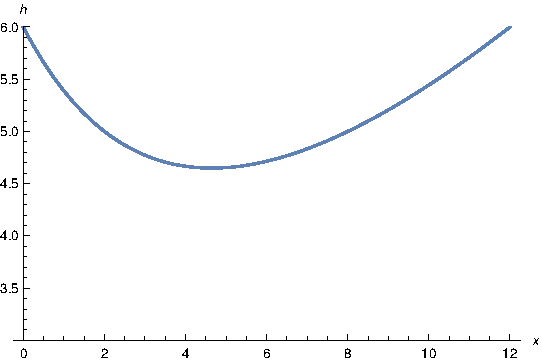
\includegraphics{Q11-1.pdf}
    \caption{$x$에 따른 $h$의 그래프}
    \label{<label>}
  \end{figure}
  \item[(라)] 질량 중심이 가장 낮은 점에 있을 때를 찾기 위해 식(\ref{eq:1-2})을 
  $x$에 대해 미분하여 0이 되도록 하는 $x$를 찾자. 즉,
  \begin{align}
    \frac{dh}{dx} = \frac{MH^2m_0-2MHm_0x-m_0^2x^2}{2(MH+m_0x)^2} = 0
  \end{align}
  을 만족하는 $x$를 구해야 한다. 이는 $x$에 대한 2차 방정식인,
  \begin{align}
    m_0^2x^2 +2MHm_0x -MH^2m_0 = 0 
  \end{align}
  을 푸는 것과 같다. 근의 공식을 이용하면,
  \begin{align}
    x = \frac{-MHm_0\pm\sqrt{M^2H^2m_0^2+MH^2m_0^3}}{m_0^2}
    = \frac{-MH\pm H\sqrt{M(M+m_0)}}{m_0}.
  \end{align}
  $M=1.40\times 10^{3}\,\mathrm{g}$, $H=12\,\mathrm{cm}$,
  $m_0=2.10\times 10^3\,\mathrm{g}$ 이므로,
  \begin{align}
    \begin{split}
      x_1 =& \frac{-(1.40\times 10^{3}\,\mathrm{g})(12\,\mathrm{cm}) 
      - (12\,\mathrm{cm})\sqrt{(1.40\times 10^{3}\,\mathrm{g})
      ((1.40\times 10^{3}\,\mathrm{g})
      +2.10\times 10^3\,\mathrm{g})}}{2.10\times 10^3\,\mathrm{g}}
      =-21\,\mathrm{cm}  \\
      x_2 =& \frac{-(1.40\times 10^{3}\,\mathrm{g})(12\,\mathrm{cm}) 
      + (12\,\mathrm{cm})\sqrt{(1.40\times 10^{3}\,\mathrm{g})
      ((1.40\times 10^{3}\,\mathrm{g})
      +2.10\times 10^3\,\mathrm{g})}}{2.10\times 10^3\,\mathrm{g}}
      =4.6\,\mathrm{cm}
    \end{split}
  \end{align}
  여기서 $x_1<0$은 우리가 원하는 길이가 아니다. 따라서 $x$는,
  \begin{align}
    x = 4.6\,\mathrm{cm}.
  \end{align}
  이고 $h$는 식 \eqref{eq:1-2}에 대입하여 구할 수 있다.
  \begin{align}
    \begin{split}
      h &= \frac{(1.40\times 10^{3}\,\mathrm{g})(12\,\mathrm{cm})^2
      +(2.10\times 10^3\,\mathrm{g})(4.6\,\mathrm{cm})^2}
      {2((1.40\times 10^{3}\,\mathrm{g})(12\,\mathrm{cm})
      +(2.10\times 10^3\,\mathrm{g})(4.6\,\mathrm{cm}))}  \\
      &= 4.6\,\mathrm{cm}.
    \end{split}
  \end{align}
  $h = 4.6\,\mathrm{cm}$이다.
\end{itemize}
\vspace{1cm}
\noindent {\bf 문제 2. (20 pt)}
그림 \ref{fig:2}와 같이 질량 $m$인 총알이 용수철에 달려있는 질량 $M$인
나무토막에 속도 $v$로 날아와 박혔다. 용수철 상수는 $k$이고 용수철 끝은
벽에 고정되어 있으며, 나무토막과 바닥면 사이의 마찰은 무시한다. 이때,
용수철의 최대 압축거리를 구하여라. 
\begin{figure}[ht]
  \centering
\includegraphics[scale=0.4]{Qfig11-2-20220406.png}
  \caption{문제 2}
  \label{fig:2}
\end{figure}

\noindent {\bf 풀이 : }
날아오는 총알의 역학적 에너지 $E_i$는,
\begin{align}\label{eq:2-1}
  E_i = \frac{1}{2}mv^2.
\end{align}
총알은 오직 운동에너지만 가지고 있다. 총알이 날아와서 박히면 총알의 
운동에너지가 토막의 운동에너지와 용수철의 탄성 위치에너지로 변환된다.
이 때 토막과 총알의 속력을 $v^\prime$, 용수철이 압축된 거리를 $x_1$이라 하자.
용수철, 토막, 총알이 가진 역학적 에너지의 합을 $E_1$라고 하면,
\begin{align}
E_1=\frac{1}{2}kx_1^2+\frac{1}{2}M{v^\prime}^2+\frac{1}{2}m{v^\prime}^2
\end{align}
용수철이 최대로 압축되는 순간, 토막과 총알은 정지한다. 즉 총알과 토막의
운동에너지는 0이고 모든 에너지가 용수철의 탄성 위치에너지로 변환된다. 
이 때 압축된 거리를 $x$, 용수철, 토막, 총알이 가진 역학적 에너지의 합을 
$E_f$라고 하면,
\begin{align}\label{eq:2-3}
  E_f = \frac{1}{2}kx^2
\end{align}
이다. 역학적 에너지는 보존되어야 하므로,
\begin{align}
  E_i = E_1 = E_f
\end{align}
이고 식 (\ref{eq:2-1})과 식 (\ref{eq:2-3})에 의해,
\begin{align}
  \frac{1}{2}mv^2=\frac{1}{2}kx^2,\,\,\,x=\sqrt{\frac{m}{k}}v.
\end{align}
용수철이 최대로 압축되는 거리는,
\begin{align}
  x=\sqrt{\frac{m}{k}}v
\end{align}
이다.
\vspace{1cm}

\noindent {\bf 문제 3. (40pt)} 
그림~\ref{fig:3}에서 질량이 2.00 kg인 토막 1이 오른쪽으로 10 m/s의
속력으로 움직이고 질량이 5.00 kg인 토막 2는 오른쪽으로 3.00 m/s의
속력으로 움직인다. 표면에는 마찰력이 없고, 토막 2에는 용수철 상수가
$1.120\times 10^3$ N/m인 용수철이 고정되어 있다. 이 두 토막이 충돌할
때, 용수철은 두 토막의 속도가 같아지는 순간에 최대로
압축된다. 이 용수철의 최대 압축거리를 구하여라. 
\begin{figure}[ht]
  \centering
   \includegraphics[scale=0.4]{Qfig11-4-20210406.png}
  \caption{문제 3}
  \label{fig:3}
\end{figure}

\noindent {\bf 풀이 : } 토막 1의 질량과 초기 속력을 $m_1$, $v_1$,
토막 2의 질량과 초기 속력을 $m_2$, $v_2$라 하자. 용수철이 압축되기 전 
두 토막의 역학적 에너지의 합 $E_i$는 다음과 같다.
\begin{align}\label{eq:3-1}
  E_i = \frac{1}{2}m_1v_1^2+\frac{1}{2}m_2v_2^2.
\end{align}
용수철이 최대로 압축되었을 때 두 토막의 속력을 $v$, 압축된 거리를 $x$라고 
한다면 이 때 두 토막의 역학적 에너지와 용수철의 탄성 위치에너지의 합 $E_f$는,
\begin{align}\label{eq:3-2}
  E_f = \frac{1}{2}m_1v^2+\frac{1}{2}m_2v^2+\frac{1}{2}kx^2
\end{align}
이다. 역학적 에너지는 보존되어야 하므로,
\begin{align}\label{eq:3-3}
  E_i = E_f,\,\,\,\frac{1}{2}m_1v_1^2+\frac{1}{2}m_2v_2^2
  = \frac{1}{2}m_1v^2+\frac{1}{2}m_2v^2+\frac{1}{2}kx^2.
\end{align}
한편 운동량 또한 보존되어야 하므로,
\begin{align}\label{eq:3-4}
  m_1v_1+m_2v_2 = m_1v+m_2v,\,\,\,v=\frac{m_1v_1+m_2v_2}{m_1+m_2}
\end{align}
이다. 식 (\ref{eq:3-3})에 대입하면 다음과 같다.
\begin{align}
  \begin{split}
    \frac{1}{2}m_1v_1^2+\frac{1}{2}m_2v_2^2
    &= \frac{1}{2}(m_1+m_2){\left(\frac{m_1v_1+m_2v_2}{m_1+m_2}\right)}^2
    +\frac{1}{2}kx^2  \\
    &=\frac{1}{2}\frac{(m_1v_1+m_2v_2)^2}{m_1+m_2}
    +\frac{1}{2}kx^2.
  \end{split}
\end{align}
$x$에 대해 정리하면,
\begin{align}
  \begin{split}
    x &= \sqrt{\frac{1}{k}\left(
      m_1v_1^2+m_2v_2^2-\frac{(m_1v_1+m_2v_2)^2}{m_1+m_2}
      \right)}  \\
      &= \sqrt{\frac{1}{k}\left(
        \frac{m_1^2v_1^2+m_2^2v_2^2+m_1m_2(v_1^2+v_2^2)}{m_1+m_2}
        -\frac{m_1^2v_1^2+m_2^2v_2^2+2m_1m_2v_1v_2}{m_1+m_2}
        \right)}  \\
        &=\sqrt{\frac{1}{k}\left(
          \frac{m_1m_2}{m_1+m_2}
          \right)}(v_1-v_2).
      \end{split}
\end{align}
이다. $m_1=$ 2.00 kg, $m_2=$ 5.00 kg, $v_1=$ 10 m/s, $v_2=$ 3.00 m/s이고 
$k=$ $1.120\times 10^3$ N/m이므로,
\begin{align}
  \begin{split}
    x &= \sqrt{\frac{1}{1.120\times 10^3\,\mathrm{N/m}}\left(
      \frac{(2.00\,\mathrm{kg})(5.00\,\mathrm{kg})}
      {2.00\,\mathrm{kg}+5.00\,\mathrm{kg}}
      \right)}(10\,\mathrm{m/s}-3.00\,\mathrm{m/s}) \\
      &= 0.25\,\mathrm{m}.
  \end{split}
\end{align}
용수철의 최대 압축거리는 $0.25\,\mathrm{m}$이다.
\vspace{1cm}

\noindent {\bf 문제 4. (20pt)}
질량이 0.500 kg의 강철공이 길이 70.0 cm이고 한쪽 끝이 벽에 고정된 줄에
매달려 있다. 그림~\ref{fig:4}처럼 수평상태에서 공을 놓았다. 공이
내려오다가 최저점에서 질량이 2.50 kg인 정지해있는 강철 토막과
충돌하였다. 토막과 공의 표면 사이에 쓸림이 없다고 하자. 
탄성충돌할 때 충돌 직후의 
\begin{figure}[ht]
  \centering
  \includegraphics[scale=0.5]{Qfig11-4_20220406.png}
  \caption{문제 4}
  \label{fig:4}
\end{figure}
\begin{itemize}
\item[(가)] 공과 
\item[(나)] 토막의 속력을 각각 구하여라. 
\end{itemize}
\noindent {\bf 풀이 : } 
\begin{itemize}
  \item[(가)] 공이 가진 초기 역학적 에너지를 $E_i$, 충돌 전 최저점에서 
공의 역학적 에너지를 $E_f$라고 하자. 최저점에서 공의 위치에너지를 0이라고 하면,
\begin{align}
  E_i = mgh,\,\,\, E_f=\frac{1}{2}mv^2.
\end{align}
역학적 에너지는 보존되어야 하므로,
\begin{align}\label{eq:4-1}
  E_i = E_f,\,\,\, mgh=\frac{1}{2}mv^2
\end{align}
이다. 공과 토막은 탄성충돌하였으므로 운동량과 에너지가 보존된다. 
탄성충돌 이후 공의 속력과 질량을 $v_1$, $m_1$ 토막의 속력과 질량을 $v_2$, $m_2$ 라고 
하자. 운동량 보존 법칙에 의해,
\begin{align}\label{eq:4-2}
  m_1v+0 = m_1v_1+m_2v_2,\,\,\,m_1(v-v_1)=m_2v_2
\end{align}
이고 에너지 보존 법칙에 의해,
\begin{align}\label{eq:4-3}
  \frac{1}{2}m_1v^2+0 = \frac{1}{2}m_1v_1^2+\frac{1}{2}m_2v_2^2
  ,\,\,\,  m_1(v^2-v_1^2) =m_2v_2^2
\end{align}
이다. 식 (\ref{eq:4-2})를 식 (\ref{eq:4-3})에 대입하면,
\begin{align}
  \begin{split}
    m_1(v^2-v^2_1)=m_1(v-v_1)(v+v_1)=m_2v_2(v+v_1)=m_2v_2^2
  \end{split}
\end{align}
이고 따라서,
\begin{align}\label{eq:4-4}
  v+v_1 = v_2
\end{align}
이다. 식 (\ref{eq:4-2})에 대입하고 $v_1$에 대해 정리하면,
\begin{align}
  v_1 = \frac{m_1-m_2}{m_1+m_2}v.
\end{align}
이다. 식 (\ref{eq:4-1})에 의해,
\begin{align}
  v = \sqrt{2gh}.
\end{align}
따라서 $v_1$은 다음과 같다.
\begin{align}
  \begin{split}
    v_1 &= \frac{m_1-m_2}{m_1+m_2}\sqrt{2gh}.
  \end{split}
\end{align}
$m_1= 0.500\,\mathrm{kg}$, $m_2 = 2.50\,\mathrm{kg}$, 
$h=7.00\times 10^{-1}\,\mathrm{m}$ 이므로 $v_1$은 다음과 같다.
\begin{align}
  \begin{split}
    v_1 &= \frac{(0.500\,\mathrm{kg}-2.50\,\mathrm{kg})}
    {(0.500\,\mathrm{kg}+2.50\,\mathrm{kg})}
    \sqrt{2(9.80\,\mathrm{m/s^2})(7.00\times 10^{-1}\,\mathrm{m})}  \\
    &= -2.47\,\mathrm{m/s}.
  \end{split}
\end{align}
\item[(나)] 식 (\ref{eq:4-4})에 의해,
\begin{align}
  \begin{split}
    v_2 &= \sqrt{2gh}+v_1  \\
    &=\sqrt{2(9.80\,\mathrm{m/s^2})(7.00\times 10^{-1}\,\mathrm{m})}
    -2.47\,\mathrm{m/s} \\
    &=1.23\,\mathrm{m/s}.
  \end{split}
\end{align}
탄성충돌 후 토막은 $1.23\,\mathrm{m/s}$의 속력으로 움직인다.
\end{itemize}
\end{document}